\documentclass{beamer}

\usetheme{Luebeck}
\usecolortheme{dove}

\usepackage{tikz}
\usetikzlibrary{arrows,automata} 

\begin{document}
\title{Constructive Formalization of Regular Languages}  
\author[Jan-Oliver Kaiser]{Jan-Oliver Kaiser \\{\small Advisors: Christian Doczkal, Gert Smolka }\\{\small Supervisor: Gert Smolka}}

\date{\today} 


\begin{frame}
    \titlepage
\end{frame}

\begin{frame}
    \tableofcontents
\end{frame}

\begin{frame}
    \section{Quick recap}

    Our roadmap:

    \begin{enumerate}
        \item RE $\Rightarrow$ FA (\textbf{DONE})
        \item Emptiness test on FA (\textbf{Easy})
        \item RE equivalence (\textbf{Follows from 1 and 2})
        \item FA $\Rightarrow$ RE
        \item Myhill-Nerode
    \end{enumerate}

\end{frame}

\section{Finite automata to regular expressions}
\subsection*{Difficulty}
\begin{frame}

    \large{\textbf{Finite automata to regular expressions}}

    \begin{itemize}
        \item
            Converting REs to FAs is straight forward and there is really only one algorithm (with slight variations).

            \pause

        \item
            Converting FAs to REs is complicated and there are at least three general algorithms.
    \end{itemize}

    \pause

    \textbf{Why is that?}

\end{frame}

\begin{frame}
    \textbf{My intuition:} 
    \begin{itemize}
        \item
            Converting REs to FAs is done by structural recursion on a \textbf{tree}. The result is a \textbf{flat structure}.

            \pause

        \item
            Converting FAs to REs \textbf{can not be done} by structural recursion. There is no \textbf{recursive structure} in FAs. But somehow we need to construct a \textbf{tree structure}.
    \end{itemize}



\end{frame}

\subsection*{Overview}
\begin{frame}

    \textbf{Three methods (+ variations):}

    \begin{enumerate}
        \item Transitive Closure
        \item State Removal
        \item Brzozowski Algebraic Method
    \end{enumerate}

\end{frame}

\section{Transitive Closure}
\subsection*{Approach}
\begin{frame}

    \large{\textbf{Transitive Closure}} \\

    \textbf{Given}: DFA $A$ = $(\Sigma, Q, s_0, F \subseteq Q, \delta)$.

    \textbf{Idea}: Construct regexps $r_f$ for every final states $f \in F$ s.t. \\$r_f$ matches all words which A accepts with final state $f$. \\

    $\, \Rightarrow \mathcal{L}(A) = \mathcal{L}(\sum_{f \in F} r_f)$

    \vspace{5 mm}

    \textbf{How do we construct $r_f$?} 

\end{frame}

\subsection*{Algorithm}
\begin{frame}

    We generalize the idea of $r_f$ to $R^k_{i j}$ which matches all words with which lead from state $i$ to $j$ while passing only through states with index smaller than $k$.

    \begin{enumerate}
        \item 
            Merge multiple edges between states to one unified edge.
        \item
            Construct regexp $R^k_{i j}$ recursively:

            \begin{description}

                \item[$R^0_{i j}$]
                    $ := \begin{cases} 
                        r & \mbox{if } i \neq j \wedge i \mbox{ has edge } r \mbox{ to j}  \\
          \varepsilon + r & \mbox{if } i = j \wedge i \mbox{ has edge } r \mbox{ to j}  \\
                \emptyset & \mbox{otherwise}
                    \end{cases}
                    $ 

                \item[$R^k_{i j}$]
                    $ := R^{k-1}_{i k} R^{k-1}_{k k} R^{k-1}_{k j} + R^{k-1}_{i j}$

            \end{description}

    \end{enumerate}

    $\Rightarrow \mathcal{L}(A) = \mathcal{L}(\sum_{f \in F} r_f) = \mathcal{L}(\sum_{f \in F} R^{|Q|}_{0 f})$

\end{frame}

\subsection*{Properties}
\begin{frame}
    \begin{description}
        \item[\textbf{Formalization}:] \hfill \\
            Easier than the other methods.\\
            The recursive definition translates quite well.\\
            Some details are quite challenging.

        \item[\textbf{Efficiency}:] The resulting regular expressions are huge.

        \item[\textbf{Complexity}:]
            $O(n^3)$ in the number of states.
    \end{description}
\end{frame}

\section{State Removal}
\subsection*{Approach}
\begin{frame}
    \textbf{State Removal}    

    \textbf{Given}: FA $A$ = $(\Sigma, Q, s_0, F \subseteq Q, \delta)$.

    \textbf{New concept}: Automata that have transitions labeled by RE.

    \textbf{Idea}: Remove states until there are two or less states remaining. Update the remaining states' transitions by incorporating the "lost" paths.


\end{frame}

\subsection*{Algorithm}
\begin{frame}
    \textbf{Remove $q$ from}\\

    \begin{figure}
        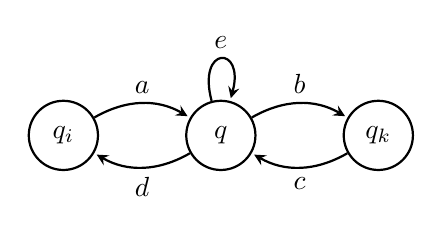
\begin{tikzpicture}[shorten >=1pt,node distance=2cm,>=stealth,thick]
            \node[state] (1) {$q_i$};
            \node[state] (2) [right of=1] {$q$};
            \node[state] (3) [right of=2] {$q_k$};
            \draw [->] (1) to[bend left] node[auto] {$a$} (2);
            \draw [->] (2) to[bend left] node[auto] {$b$} (3);
            \draw [->] (2) to[loop above] node[auto] {$e$} (2);
            \draw [->] (3) to[bend left] node[auto] {$c$} (2);
            \draw [->] (2) to[bend left] node[auto] {$d$} (1);
        \end{tikzpicture}
        \\
    \end{figure}

    \pause

    \textbf{to get}\\

    \begin{figure}
        \begin{tikzpicture}[shorten >=1pt,node distance=2cm,>=stealth,thick]
            \node[state] (1) {$q_i$};
            \node[state] (3) [right of=2] {$q_k$};
            \draw [->] (1) to[bend left] node[auto] {$ae^*b$} (3);
            \draw [->] (1) to[loop above] node[auto] {$ae^*d$} (1);
            \draw [->] (3) to[bend left] node[auto] {$ce^*d$} (1);
            \draw [->] (3) to[loop above] node[auto] {$ce^*b$} (3);
        \end{tikzpicture}
        \\
    \end{figure}

\end{frame}

\begin{frame}
    \textbf{Repeat until $A$ is of this form:}

    \begin{figure}
        \begin{tikzpicture}[shorten >=1pt,node distance=2cm,>=stealth,thick]
            \node[state] (1) {$q_1$};
            \node[state] (3) [right of=2, accepting] {$q_f$};
            \draw [->] (1) to[bend left] node[auto] {$r_2$} (3);
            \draw [->] (1) to[loop above] node[auto] {$r_1$} (1);
            \draw [->] (3) to[bend left] node[auto] {$r_3$} (1);
            \draw [->] (3) to[loop above] node[auto] {$r_4$} (3);
        \end{tikzpicture}
        \\
        $\Rightarrow \mathcal{L}(A) = \mathcal{L}(r_1^* r_2 (r_4 + r_3 r_1^* r_2)^*)$
    \end{figure}


\end{frame}

\subsection*{Caveats}
\begin{frame}
    \textbf{Caveats} \\
    \begin{itemize}
        \item
            It looks like we only need to update two edges. \\
            \pause
            In reality, there can be $|Q|-1$ states connected to $q$.
            \pause
        \item
            What about final states?\\
            \pause
            Introduce a new final state without any outgoing edges. \\
            Introduce $\varepsilon$ transitions from all other final states to the final new state. \\
            Make all other states non-final. \\
            Never remove the new final state.
    \end{itemize}


\end{frame}

\subsection*{Properties}
\begin{frame}
    \begin{description}
        \item[\textbf{Formalization}:] \hfill \\
            Complex.\\
            Lots of details to consider.
        \item[\textbf{Efficiency}:] 
            The resulting regular expressions are big.\\
            They can be made small in special cases (e.g., acyclic automata).

        \item[\textbf{Complexity}:]
            $O(n^3)$ in the number of states.\\
            Less in special cases (e.g. $O(n^2 log n)$ for acyclic automata).
    \end{description}
\end{frame}

\section{Brzozowski Algebraic Method}
\subsection*{Approach}
\begin{frame}
    \textbf{Brzozowski Algebraic Method}

    \textbf{Given}: FA $A$ = $(\Sigma, Q, q_0, F \subseteq Q, \delta)$.\\
    \textbf{Idea}: Retrieve a RE for FA by solving a system of equations determined by $\delta$.

\end{frame}

\subsection*{Algorithm}
\begin{frame}
    \textbf{Construct system of equations}:

    \begin{equation}
        \begin{array}{lcl} 
            r_0 & = & \displaystyle\sum\limits \{ \, a \, r_i \, | \, a \, \in \, \Sigma, \, 0 \, \leq i < \, |Q|, \, (q_0, a, r_i) \in \delta \} \\ 
           \vdots &  = & \vdots \\
            r_k & = & \displaystyle\sum\limits \{ \, a \, r_i \, | \, a \, \in \, \Sigma, \, 0 \, \leq i < \, |Q|, \, (q_k, a, r_i) \in \delta \} \\ 
           \vdots &  = & \vdots \\
        r_{|Q|-1} & = & \displaystyle\sum\limits \{ \, a \, r_i \, | \, a \, \in \, \Sigma, \, 0 \, \leq i < \, |Q|, \, (q_{|Q|-1}, a, r_i) \in \delta \}

        \end{array}
    \end{equation}
    $\, \Rightarrow \mathcal{L}(A) = \mathcal{L}(r_0)$
\end{frame}

\begin{frame}
\end{frame}

\end{document}
